\chapter{Operational Amplifier }
\section{Introduction}
An operational amplifier is a direct-coupled high-gain amplifier usually consisting of one or more differential amplifiers.\\ The operational amplifier is a versatile device that can be used to amplify dc as well as ac input signals and was originally designed for performing mathematical operations such as addition, subtraction, multiplication, and integration. Thus the name operational amplifier stems from its original use for these mathematical operations and is abbreviated to $o p-a m p$. With the addition of suitable external feedback components, the modern day op-amp can be used for a variety of applications, such as ac and dc signal amplification, active filters, oscillators, comparators, regulators, and others.

\begin{figure}[H]
	\centering
	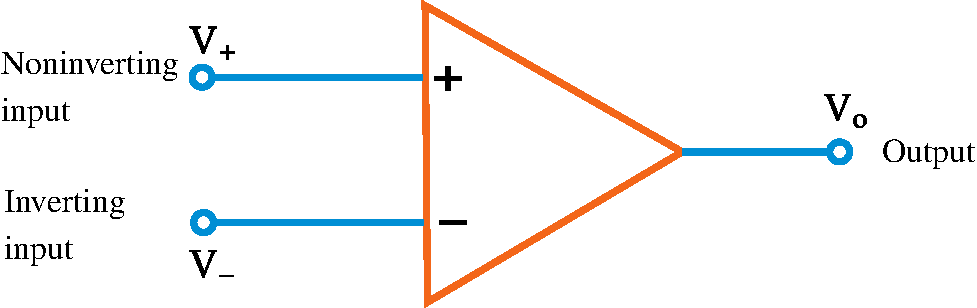
\includegraphics[height=2.2cm,width=7cm]{Opamp schematic}
	\caption{Schematic diagram of an an op-amp}
	\label{Opamp schematic}
\end{figure}
$\left. \right. $\\
 A  schematic diagram of an an op-amp is shown in the figure.\ref{Opamp schematic}. \\
  For  simplicity, power supply and other pin connections are omitted. Since the input differential amplifier stage of the op-amp is designed to be operated in the differential mode, the differential inputs are designated by the $(+)$ and $(-)$ notations. The $(+)$ input is the noninverting input. An ac signal (or dc voltage) applied to this input produces an in-phase (or same polarity) signal at the output. On the other hand, the $(-)$ input is the inverting input because an ac signal (or dc voltage) applied to this input produces an $180^{\circ}$ out-of-phase (or opposite polarity) signal at the output.
   In Figure,
   $$
   \begin{aligned}
   \mathrm{V_{+}}&=\text { Voltage at the noninverting input (volts) } \\
   \mathrm{V_{-}}&=\text { Voltage at the inverting input (volts) } \\
   \mathrm{V_{o}}&=\text { Output voltage (volts) }
   \end{aligned}
   $$
   All these voltages are measured with respect to ground.

  \section{Op-Amp characterestics}
  \subsection{Input offset voltage} 
  
   \begin{figure}[H]
   	\centering
   	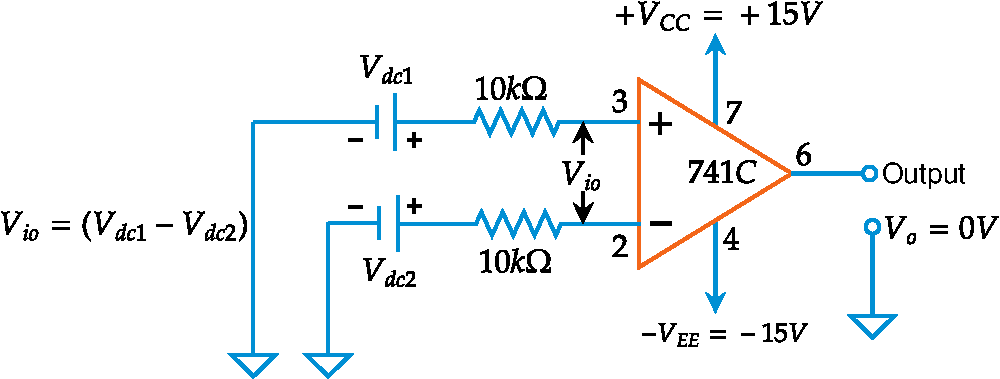
\includegraphics[height=4.5cm,width=11cm]{Input offset voltage}
   	\caption{Defining input offset voltage}
   	\label{Input offset voltage}
   \end{figure}
   \par Input offset voltage is the voltage that must be applied between the two input terminals of an op-amp to null the output, as shown in Figure.\ref{Input offset voltage}. In the figure $V_{\mathrm{dc} 1}$ and $V_{\mathrm{dc} 2}$ are dc voltages and $R_{S}$ represents the source resistance. We denote input offset voltage by $V_{i o}$. This voltage $V_{i o}$ could be positive or negative; therefore, its absolute value is listed on the data sheet. For a $741 \mathrm{C}$ the maximum value of $V_{i o}$ is $6 \mathrm{mV} \mathrm{dc}$. The smaller the value of $V_{i o}$, the better the input terminals are matched. For instance, the $714 \mathrm{C}$ precision op-amp has $V_{i o}=150 \mu \mathrm{V}$ maximum.
   \subsection{Input offset current}
   \begin{figure}[H]
   	\centering
   	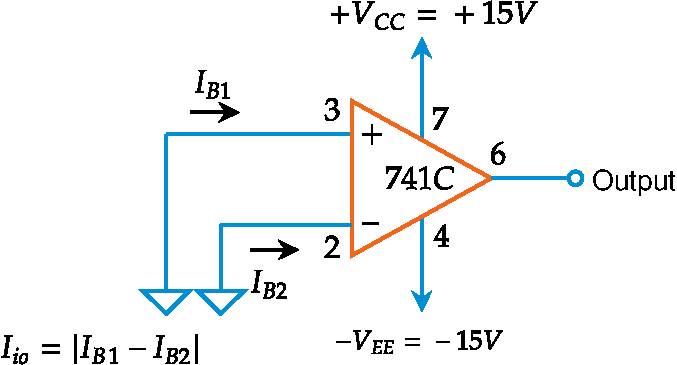
\includegraphics[height=4.5cm,width=8cm]{Input offset current}
   	\caption{Defining input offset current}
   	\label{Input offset current}
   \end{figure}
    The algebraic difference between the currents into the inverting and noninverting terminals is referred to as input offset current, $I_{i o}$. In the form of an equation,
   $$
   I_{i o}=\left|I_{B 1}-I_{B 2}\right|
   $$
   where $I_{B 1}$ is the current into the noninverting input and $I_{B 2}$ is the current into the inverting input.
   \subsection{Input bias current}
   Input bias current, $I_{B}$, is the average of the currents that flow into the inverting and noninverting input terminals of the op-amp. In equation form,
   $$
   I_{B}=\frac{I_{B 1}+I_{B 2}}{2}
   $$
   $I_{B}=500 \mathrm{nA}$ maximum for the $741 \mathrm{C}$, whereas $I_{B}$ for the precision $714 \mathrm{C}$ is $\pm 7 \mathrm{nA} .$ \\
   Note that the two input currents $I_{B 1}$ and $I_{B 2}$ are actually the base currents of the first differential amplifier stage.
   \subsection{Differential input resistance}
   Differential input resistance, $R_{i}$, (often referred to as input resistance) is the equivalent resistance that can be measured at either the inverting or noninverting input terminal with the other terminal connected to oround. For the $741 \mathrm{C}$ the input resistance is a relatively high $2 \mathrm{M} \Omega$.
   \subsection{Common Mode Rejection Ratio (CMRR)}
  \textbf{The common-mode rejection ratio (CMRR) }is defined in several essentially equivalent ways by various manufacturers. Generally, it can be defined as the ratio of the differential voltage gain $A_{d}$ to the common-mode voltage gain $A_{\mathrm{cm}} $ that is,
   \begin{equation}
   \mathrm{CMRR}=\frac{A_{d}}{A_{\mathrm{cm}}}
   \end{equation}
  
   The differential voltage gain $A_{d}$ is the same as the large-signal voltage gain $A$, which is specified on the data sheets; however, the common-mode voltage gain can be determined from  using the equation,
   \begin{equation}
  \mathrm{A}_{\mathrm{cm}}=\frac{V_\mathrm{ocm}}{V_{\mathrm{cm}}}
   \end{equation}
   $$
   \begin{aligned}
   \text{Where ,} V_\mathrm{ocm}&= \text{output common-mode voltage}\\
   V_{\mathrm{cm}}&=\text { input common-mode voltage } \\
   A_{\mathrm{cm}}&=\text { common-mode voltage gain }
   \end{aligned}
   $$
   Generally the $A_{\mathrm{cm}}$ is very small and $A_{d}=A$ is very large, therefore, the $\mathrm{CMK}$ is very large. Being a large value, CMRR is most often expressed in decibels (dB). For the $741 \mathrm{C}$, CMRR is $90 \mathrm{~dB}$ typically.
   \begin{note}
   	  \textbf{Common mode voltage:} When the same voltage is applied to both input terminals, the voltage is called a common-mode voltage, $V_{\mathrm{cm}}$, and the op-amp is said to be operating in the common-mode configuration.
   \end{note}
   \subsection{Output resistance}
   Output resistance, $R_{o}$, is the equivalent resistance that can be measured between the output terminal of the op-amp and the ground (or common point). It is $75 \Omega$ for the $741 \mathrm{C}$ op-amp.
   \subsection{Slew rate}
   Slew rate (SR) is defined as the maximum rate of change of output voltage per unit of time and is expressed in volts per microseconds. In equation form,
   $$
   \mathrm{SR}=\left.\frac{d V_{o}}{\mathrm{dt}}\right|_\mathrm{max} \mathrm{V} / \mu \mathrm{s}
   $$
   Slew rate indicates how rapidly the output of an op-amp can change in response to changes in the input frequency. The slew rate changes with change in voltage gain and is normally specified at unity $(+1)$ gain. The slew rate of an op-amp is fixed; therefore, if the slope requirements of the output signal are greater than the slew rate, then distortion occurs. Thus slew rate is one of the important factors in selecting the op-amp for ac applications, particularly at relatively high frequencies.\\
    One of the drawbacks of the $ 741 \mathrm{C}$ is its low slew rate $(0.5 \mathrm{~V} / \mu \mathrm{s})$ 
   \section{The ideal Op-Amp} 
   An ideal op-amp would exhibit the following electrical characteristics,
   \begin{enumerate}
   	\item  Infinite voltage gain $A$.
   	\item Infinite input resistance $R_{i}$ so that almost any signal source can drive it and there is no loading of the preceding stage.
   	\item Zero output resistance $R_{o}$ so that the output can drive an infinite number of other devices.
   	\item Zero output voltage when input voltage is zero.
   	\item Infinite bandwidth so that any frequency signal from 0 to $\infty \mathrm{Hz}$ can be amplified without attenuation.
   	\item Infinite common-mode rejection ratio so that the output common-mode noise voltage is zero.
   	\item Infinite slew rate so that output voltage changes occur simultaneously with input voltage changes.
   \end{enumerate}
   There are practical op-amps that can be made to approximate some of these characteristics using a negative feedback arrangement.
   \newpage
   \begin{abox}
   Practice Set- 1
   \end{abox}
\begin{enumerate}
	\item d
\end{enumerate}
     \newpage
  \begin{abox}
  	Practice Set- 2
  \end{abox}
  \begin{enumerate}
  	\item d
  \end{enumerate} 